\documentclass[12pt,letterpaper]{beamer}
\usetheme{Copenhagen}
\usecolortheme{seahorse}
\setbeamertemplate{section in toc}{\inserttocsection}

\usepackage[utf8]{inputenc}
\usepackage{amsmath}
\usepackage{amsfonts}
\usepackage{amssymb}
\usepackage{graphicx}
\graphicspath{ {./images/} }
\usepackage{multirow}
\usepackage{hyperref}
\hypersetup{
    colorlinks=true,
    linkcolor=blue,
    filecolor=magenta,      
    urlcolor=cyan,
    pdftitle={Overleaf Example},
    pdfpagemode=FullScreen,
}
\title[Robotics I]
{ENGR 3421: ROBOTICS I}
\subtitle{Introduction to Linux}

\author[Zhang, Lin]
{Dr. Lin Zhang}
\institute[UCA] % (optional)
{
  Department of Physics and Astronomy\\
  University of Central Arkansas
}
\date[Robotics1 2021] % (optional)
{September 14, 2021}
\logo{
\includegraphics[height=1cm]{../images/uca_bear_logo.png}}


%End of title page configuration block
%------------------------------------------------------------

%------------------------------------------------------------
%The next block of commands puts the table of contents at the beginning of each section and highlights the current section:

\AtBeginSection[]
{
  \begin{frame}
    \frametitle{Outline}
    \tableofcontents[currentsection]
  \end{frame}
}
%------------------------------------------------------------

\begin{document}

%The next statement creates the title page.
\frame{\titlepage}

%---------------------------------------------------------
%This block of code is for the table of contents after the title page
\begin{frame}
\frametitle{Outline}
\tableofcontents
\end{frame}
%---------------------------------------------------------

\section{Story of Linux}

\begin{frame}{Story of Linux}
    {\centering
        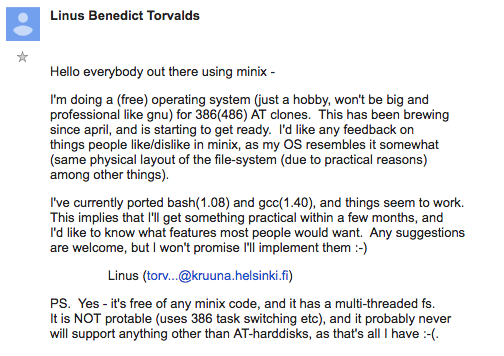
\includegraphics[width=0.8\linewidth]{linus_torvald_first_linux_email}
    }
\end{frame}

\begin{frame}{Linux Distros}
    Distro is a complete operating system based on the Linux kernel that contains a bunch of packages and libraries.
    \begin{itemize} 
        \item Debian(for home users)
        \item Redhat(for enterprises)
        \item Slackware
        \item Android
    \end{itemize} 
\end{frame}

\section{Linux Command Line}
\begin{frame}{Linux Command Line}
    The Linux command line is a text interface to your computer. 
    \begin{block}{Note}
        Check out this \href{https://ubuntu.com/tutorials/command-line-for-beginners}{tutorial}
    \end{block}
    
    \begin{itemize}
        \item Opening a terminal
        \item Changing directories
        \item Creating folders and files
        \item Manipulating files
        \item The superuser
    \end{itemize}

\end{frame}

\begin{frame}{Package Management}
    The package management system installs, upgrades, configures and removes software. 
    \begin{itemize}
        \item apt
        \item dpkg
    \end{itemize}

\end{frame}


\end{document}

